% ----------------------------------------------------------
\chapter{Referencial Teórico}\label{cap:referencial-teorico}
% ----------------------------------------------------------
\section{Metodologias Tradicionais}
As metodologias tradicionais, também conhecidas como pesadas ou orientadas a documentação, foram desenvolvidas em um contexto de desenvolvimento de software que era significativamente diferente do ambiente atual (ROYCE, 1970). Dentro desse contexto, podemos destacar as metodologias de desenvolvimento em cascata (waterfall) e outros processos de desenvolvimento que se baseiam nesse modelo (TELES, 2004) como exemplos de abordagens tradicionais no desenvolvimento de software.

As metodologias clássicas desenvolvidas para apoiar os processos de Engenharia de Software, assim como as definições de papéis e estruturas organizacionais estabelecidas desde as primeiras Fábricas de Software na década de 70 (CUSUMANO, 1991), compartilham semelhanças significativas com as estruturas organizacionais baseadas no Taylorismo, que envolvem a divisão de tarefas e a atribuição a profissionais especializados. Essas semelhanças persistem em muitas equipes de desenvolvimento de software em diversos ambientes empresariais até hoje (SENAI - 2004).

O termo "tradicional" é utilizado para descrever metodologias ou processos baseados no modelo clássico, como o Modelo em Cascata. Essas abordagens são caracterizadas por uma separação rígida das fases do projeto, que incluem Levantamento de Requisitos, Análise, Desenho, Implementação, Testes e Implantação. Cada fase possui suas próprias peculiaridades e depende da conclusão da fase anterior. Essas metodologias também seguem algumas premissas, como linearidade, determinismo, especialização, foco na execução e aumento exponencial dos custos de alteração.

Ao examinarmos o paradigma clássico do ciclo de desenvolvimento de software, representado pelo modelo cascata (figura 1), podemos observá-lo como um processo linear e sequencial, semelhante às linhas de montagem industrial. Ele estabelece etapas distintas e progressivas, desde a identificação dos requisitos até os testes e a entrega final do software pronto.

Nas metodologias tradicionais, o processo de desenvolvimento é dividido em duas etapas principais: concepção e construção. Na fase de concepção, há uma interação intensa com o cliente e um grande esforço é dedicado à identificação precisa das necessidades, a fim de evitar surpresas ou mudanças durante a fase de construção. Essa fase de concepção é considerada crucial para o sucesso do projeto, pois sua qualidade e abrangência influenciam diretamente nos resultados finais (PONTES, 2018).

Embora tenham sido adaptadas ao longo do tempo para se adequarem às necessidades de otimização do processo e permitirem entregas parciais e iterativas, as metodologias tradicionais ainda mantêm as etapas básicas do Modelo Cascata em grande parte dos processos metodológicos atuais. Essas metodologias enfatizam a documentação e dedicam um esforço significativo ao levantamento, análise e especificação formal dos requisitos do sistema nas etapas iniciais do

\begin{figure}[htb]
	\caption{\label{fig:Fig_1}Modelo Cascata (Waterfall).}
	\begin{center}
		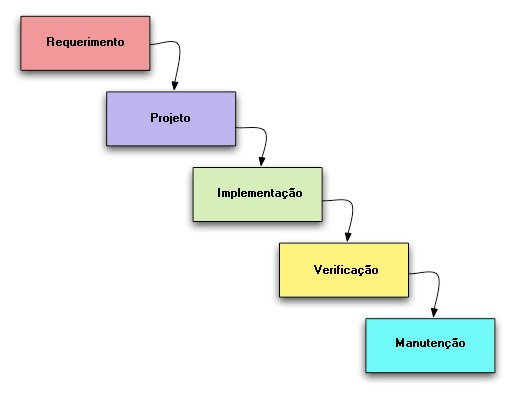
\includegraphics{figuras/Imagem1.jpg}
	\end{center}
	\fonte{https://www.ivoryit.com.br/2022/05/06/metodologias-de-desenvolvimento-de-software-conheca-as-principais/}
\end{figure}

desenvolvimento, com a expectativa de que esses requisitos possam ser mantidos estáveis e imutáveis (CORDEIRO, 2014).

Nas metodologias tradicionais, se surgirem imprevistos durante a fase de construção, isso pode resultar em retrabalho e atrasos no projeto, impactando o preço, prazo e qualidade do produto final. Isso pode gerar conflitos com o cliente, que pode se sentir insatisfeito e o sistema pode não atender plenamente às suas necessidades. Além disso, a falta de interação com o cliente durante a fase de construção impede que correções ou modificações no escopo do projeto sejam feitas. As metodologias tradicionais são mais adequadas quando os requisitos são estáveis e previsíveis, o que geralmente não ocorre no desenvolvimento de software, onde os requisitos tendem a ser altamente mutáveis (PONTES, 2018).

De acordo com Caetano (2010), em alguns projetos as metodologias tradicionais podem limitar os desenvolvedores, mantendo-os presos a requisitos desatualizados que não atendem às necessidades reais dos clientes. Por isso, muitas empresas de desenvolvimento de software estão buscando métodos alternativos que sejam mais adequados para lidar com mudanças e necessidades dos clientes. A combinação de agilidade, adaptabilidade e qualidade do produto final é essencial para garantir a satisfação do cliente. Ao adotar abordagens mais ágeis, as empresas podem responder de forma mais eficiente às mudanças e entregar produtos que atendam melhor às expectativas dos clientes.

\section{Metodologias Ágeis}
As metodologias ágeis surgiram como uma resposta às metodologias tradicionais mais pesadas e ao modelo em cascata, buscando oferecer abordagens mais flexíveis e adaptáveis ao desenvolvimento de software (ABRAHAMSSON, 2003). Ludvig e Reinert (2007) citam que elas surgiram como alternativas ao Modelo Tradicional em Cascata, que apresentava limitações em lidar com mudanças e necessidades do mercado. Essas metodologias representam uma nova classe de abordagens que enfatizam a colaboração, a comunicação e a entrega incremental, permitindo uma maior capacidade de resposta a mudanças e uma maior satisfação do cliente (FOWLER, 2005; HILMAN, 2004).

Uma característica fundamental das metodologias ágeis é sua abordagem adaptativa em vez de preditiva. Essas metodologias reconhecem a dificuldade e o alto custo de tentar prever e planejar todos os aspectos do desenvolvimento de um projeto de software. Em vez disso, elas valorizam a capacidade de se adaptar a novos fatores e mudanças ao longo do processo. O foco está em receber, avaliar e responder às mudanças de forma ágil e eficiente. Ao trabalhar com feedback constante, as metodologias ágeis permitem uma rápida adaptação aos requisitos em constante evolução. Isso contrasta com as metodologias tradicionais, que tendem a enfrentar dificuldades para lidar com mudanças significativas. Além disso, as metodologias ágeis destacam-se por suas entregas iterativas e frequentes de partes funcionais do software. Essa abordagem permite que o cliente acompanhe o progresso do projeto de forma contínua, evitando surpresas desagradáveis ao final do desenvolvimento (SOARES, 2004).

A utilização dos métodos ágeis permite a elaboração de planos flexíveis, nos quais é possível realizar alterações no produto em qualquer fase, inclusive após a finalização, conforme apontado por Gustavsson e Rönnlund (2013). Além disso, esses métodos empregam ciclos interativos de curta duração, com entregas ao final de cada ciclo. Gustavsson e Rönnlund (2013) também destacam que o foco está na eficiência de equipes pequenas, independentemente do tamanho do projeto, sugerindo um número ideal de 10 pessoas. No entanto, é importante ressaltar que relatos de projetos bem-sucedidos com mais de 250 pessoas também foram registrados (Boehm \& Turner, 2004), mostrando que os métodos ágeis podem ser adaptados e aplicados com sucesso em diferentes contextos organizacionais.

De fato, os métodos ágeis têm encontrado aplicação em diversos campos, indo além do desenvolvimento de software. Estudos como o de Gustavsson e Rönnlund (2013) destacam sua utilização na indústria, enquanto Stettina et al. (2015) observaram uma mudança significativa de interesse, com o termo "gestão de carteiras ágeis" ultrapassando o termo "desenvolvimento ágil de software" no Google Trends. Isso evidencia a crescente relevância dos métodos ágeis em outras áreas, demonstrando sua adaptabilidade e valor além do contexto do software.

\subsection{Manifesto Ágil}
A popularidade do termo "Metodologias Ágeis" ganhou destaque em 2001, quando um grupo de especialistas em processos de software, representando diferentes métodos ágeis, se reuniu para discutir maneiras de melhorar o desempenho de seus projetos. Durante essa reunião, eles identificaram um conjunto comum de princípios que, quando seguidos, levavam ao sucesso dos projetos. Essa reunião resultou na criação da Agile Alliance e na elaboração do Manifesto Ágil, que apresenta filosofias, valores e princípios fundamentais para os métodos ágeis.

Entre as diversas definições existentes para os métodos ágeis, a mais aceita é aquela que os descreve como um conjunto de práticas alinhadas aos princípios do Manifesto Ágil (Beck et al., 2001). Essas práticas enfatizam a interação colaborativa com o cliente, a entrega contínua de valor, a adaptação a mudanças, a autogestão da equipe e a busca pela excelência técnica.

Ao seguir os princípios do Manifesto Ágil, as metodologias ágeis promovem uma abordagem flexível, adaptativa e colaborativa no desenvolvimento de software, visando entregar produtos de qualidade que atendam às necessidades dos clientes de forma eficiente e eficaz.

Os princípios fundamentais das metodologias ágeis abrangem a honestidade em relação ao trabalho, a eficácia das pessoas que colaboram em equipe e o foco no trabalho em conjunto. Isso implica que o grupo de desenvolvimento, composto por desenvolvedores e representantes do cliente, esteja bem-informado, seja competente e tenha autoridade para considerar possíveis ajustes às necessidades emergentes ao longo do ciclo de vida do desenvolvimento. Isso significa que os participantes estão preparados para realizar mudanças, e que os contratos existentes são estabelecidos com ferramentas que suportam e permitem tais melhorias (LEITÃO, 2010).

De acordo com Ludvig e Reinert (2007), o Manifesto Ágil não se contrapõe aos modelos utilizados na abordagem tradicional. Os métodos ágeis se baseiam no conceito de desenvolvimento incremental (SOMMERVILLE, 2003) e incorporam técnicas provenientes da Engenharia de Software. No entanto, eles não seguem o padrão proposto pelas metodologias tradicionais (HIGHSMITH, 2000).

Assim sendo, os métodos ágeis não rejeitam processos e ferramentas, a documentação, a negociação de contratos ou o planejamento. No entanto, eles destacam que esses elementos possuem importância secundária quando comparados aos indivíduos e às iterações. A ênfase recai na entrega de software executável, na colaboração e na capacidade de resposta rápida a mudanças e alterações.

\subsection{Metodologia Scrum}
O Scrum, uma metodologia ágil de desenvolvimento de software criada por Jeff Sutherland na década de 1990, tem suas bases em conceitos tradicionais da engenharia de produção, como Lean e a Teoria das Restrições, explorados por Takeuchi e Nonaka (1986) no artigo "The new product development game". Nesse artigo, é destacada a eficácia de equipes pequenas, multidisciplinares e autogerenciáveis no desenvolvimento de produtos.

O principal objetivo do Scrum é entregar software de alta qualidade por meio de uma série de intervalos de tempo fixos, chamados Sprints, que geralmente têm duração inferior a um mês (SUTHERLAND et al., 2000). Dessa forma, o foco do Sprint é maximizar o valor de negócio entregue dentro do menor prazo possível.

De acordo com Schwaber e Sutherland (2011), o Scrum é fundamentado nas teorias empíricas de controle de processo, também conhecido como empirismo. Essa abordagem reconhece que o conhecimento é adquirido por meio da experiência e da tomada de decisões baseada no que é conhecido. O Scrum se apoia em três pilares principais:

\begin{itemize}
	\item Transparência: Os aspectos relevantes do processo devem ser visíveis e compreensíveis para todos os envolvidos, garantindo a clareza e a compreensão dos resultados esperados.
	\item Inspeção: Os praticantes do Scrum devem realizar inspeções frequentes nos artefatos e no progresso do projeto, a fim de identificar quaisquer desvios indesejáveis. Essas inspeções devem ocorrer sem interferir na execução das atividades.
	\item Adaptação: Caso seja identificado que o processo está se desviando dos limites aceitáveis e que o produto final não atenderá às expectativas, é necessário realizar ajustes no processo o mais rápido possível para garantir que o resultado final seja alcançado. A adaptação contínua é essencial para minimizar desvios e maximizar a qualidade do produto.
\end{itemize}

Esses pilares do empirismo no Scrum permitem uma abordagem flexível e iterativa, na qual o processo pode ser ajustado de acordo com as necessidades e as mudanças identificadas, garantindo um maior controle e adaptabilidade ao longo do desenvolvimento do projeto.

No Scrum, existem quatro eventos principais nos quais a inspeção e a adaptação são realizadas: a Reunião de Planejamento da Sprint, o Daily Scrum (ou Reunião Diária), a Reunião de Revisão da Sprint e a Retrospectiva da Sprint. Esses eventos permitem que a equipe revise o progresso, faça ajustes e planeje as próximas etapas do projeto.

Além disso, os valores aplicados no Scrum estão diretamente alinhados com os princípios descritos no Manifesto Ágil. Sliger e Broderick (2008) descrevem esses valores em seu livro da seguinte maneira:

\begin{alineas}
	\item Compromisso: Esteja disposto a se comprometer com uma meta. No Scrum, cada pessoa tem a autoridade necessária para cumprir os compromissos assumidos.
	\item Foco: Concentre-se em fazer seu trabalho. Direcione todos os esforços e habilidades para a realização das tarefas atribuídas, sem se preocupar com distrações ou demandas externas.
	\item Transparência: O Scrum mantém todos os aspectos de um projeto visíveis para todos os envolvidos. A transparência promove a confiança e permite que todos tenham uma compreensão clara do progresso e dos desafios.
	\item Respeito: Reconheça e respeite as diferenças individuais. As pessoas têm experiências e perspectivas únicas, e é importante valorizar e respeitar a diversidade dentro de uma equipe.
	\item Coragem: Tenha coragem para se comprometer, agir, ser aberto e buscar respeito. No Scrum, é encorajado assumir riscos, enfrentar desafios e buscar constantemente melhorias.
\end{alineas}

Esses valores são fundamentais para o sucesso do Scrum, pois promovem a colaboração, a transparência e a responsabilidade individual, criando um ambiente propício para a entrega de valor contínuo e o alcance dos objetivos do projeto.

Baseado em Vieira (2014), existem 3 papéis bem definidos para o Scrum, são eles:

\begin{enumerate}
	\item Scrum Master: O Scrum Master desempenha um papel crucial na equipe ágil. Ele é responsável por garantir o cumprimento das práticas e valores do Scrum, bem como o progresso adequado do projeto. Sua função é eliminar ou mitigar quaisquer impedimentos que possam surgir e afetar a produtividade da equipe. O Scrum Master atua como um facilitador, ajudando a equipe a se auto-organizar e a melhorar continuamente seu desempenho.
	\item Product Owner: O Product Owner é o responsável pelo gerenciamento das atividades a serem desenvolvidas, que são registradas no Product Backlog. Ele desempenha um papel crucial na definição das prioridades das atividades e na tomada de decisões relacionadas ao produto. O Product Owner trabalha em colaboração com a equipe Scrum, participando da estimativa do esforço de desenvolvimento e garantindo que o produto atenda às necessidades do cliente e agregue valor ao negócio.
	\item Scrum Team: A equipe Scrum é o grupo de desenvolvimento responsável por implementar as atividades do projeto. Essa equipe é multidisciplinar e auto-organizada, o que significa que possui todas as habilidades necessárias para realizar o trabalho e é capaz de se planejar e gerenciar internamente. A equipe é autônoma e colaborativa, trabalhando em conjunto para atingir os objetivos estabelecidos para cada Sprint.
\end{enumerate}

Ainda baseando em Vieira (2014), a metodologia adota uma série de práticas de gestão para lidar com a imprevisibilidade e complexidade inerentes aos processos. Como:

\begin{enumerate}
	\item Product Backlog: É uma lista dinâmica e prioritária de todas as funcionalidades, requisitos e melhorias desejadas para o produto. É constantemente atualizada e refinada pelo Product Owner, com base no conhecimento atual e nas necessidades do cliente.
	\item Effort Estimation: É o processo de avaliar o tempo e o esforço necessário para concluir cada item do Product Backlog. O time, juntamente com o Product Owner e o Scrum Master, realiza essa estimativa, levando em consideração a complexidade, o risco e a dependência de outros itens.
	\item Sprint: É um período de tempo fixo, geralmente de duas a quatro semanas, durante o qual a equipe trabalha para entregar um conjunto de funcionalidades priorizadas do Product Backlog. É uma unidade de trabalho e entrega dentro do projeto Scrum.
	\item Sprint Planning Meeting: É uma reunião realizada no início de cada Sprint, na qual o time, o Scrum Master e o Product Owner se reúnem para definir quais itens do Product Backlog serão incluídos na Sprint e como eles serão implementados. O resultado dessa reunião é o Sprint Backlog.
	\item Sprint Backlog: É uma lista de tarefas ou atividades específicas que foram selecionadas para serem concluídas durante a Sprint. É uma visão mais detalhada do trabalho a ser realizado, derivado do Product Backlog. O Scrum Master é responsável por garantir que o Sprint Backlog seja mantido intacto durante o Sprint.
	\item Daily Scrum: É uma reunião diária realizada pela equipe, facilitada pelo Scrum Master, na qual cada membro compartilha o que foi feito desde a última reunião, o que será feito até a próxima e quaisquer obstáculos ou impedimentos que estão enfrentando. O objetivo é manter todos alinhados e identificar rapidamente quaisquer problemas que possam afetar o progresso do trabalho.
	\item Sprint Review Meeting: É uma reunião realizada no final de cada Sprint, na qual a equipe apresenta os resultados alcançados ao Product Owner, aos gerentes e aos clientes. É uma oportunidade de demonstrar as funcionalidades concluídas e receber feedback. Como resultado dessa reunião, o Product Backlog pode ser ajustado e atualizado com base no aprendizado adquirido durante o Sprint.
\end{enumerate}

\subsection{Metodologia XP – Extreme Programming}
Extreme Programming (XP) é uma abordagem ágil de desenvolvimento de software que busca combinar rapidez, produtividade e qualidade de forma simples, atendendo às necessidades do cliente. Essa metodologia é especialmente adequada para projetos em que os requisitos estão sujeitos a mudanças constantes (PONTES, 2018).

Também segundo Pontes (2018), a metodologia XP é especialmente adequada para projetos em que os requisitos estão sujeitos a mudanças constantes. Seu principal objetivo é gerar o máximo valor possível para o cliente em um curto espaço de tempo. Durante esse período, o cliente tem a oportunidade de analisar o produto recebido e verificar se atende às suas expectativas após o seu uso.

De acordo com Beck (2004), o criador da Extreme Programming (XP), essa metodologia ágil é especialmente adequada para equipes de desenvolvimento de software de tamanho médio e pequeno. Ela se destina a lidar com situações em que os requisitos para o projeto são vagos e sujeitos a mudanças constantes.

Extreme Programming é uma metodologia que se baseia em valores e práticas visando garantir a versatilidade e a satisfação do cliente com o produto final. Os valores fundamentais do XP são:

\begin{enumerate}
	\item Comunicação: A comunicação clara e objetiva entre o cliente e a equipe é essencial para o sucesso do projeto utilizando XP. Uma comunicação eficiente permite compreender as necessidades e expectativas do cliente, além de facilitar o alinhamento e a tomada de decisões ao longo do processo de desenvolvimento.
	\item Simplicidade: O XP promove a busca pela simplicidade em todas as etapas do desenvolvimento. A ideia é fazer as coisas da forma mais simples possível, priorizando soluções funcionais e evitando a complexidade desnecessária. Dessa forma, o cliente pode obter rapidamente as funcionalidades desejadas, sem excesso de complicação.
	\item Feedback: O cliente desempenha um papel ativo no XP, aprendendo continuamente com o produto em desenvolvimento. O feedback constante proporciona a oportunidade de tomar decisões informadas sobre a priorização de atividades e ajustes nos requisitos. Isso permite que o cliente verifique se o produto está atendendo às suas expectativas e necessidades.
	\item Coragem: A coragem é encorajada no XP para enfrentar desafios e promover melhorias. Práticas como testes unitários, integração contínua e programação em par aumentam a confiança da equipe. Isso permite que se tenha coragem para refatorar o código existente, investir tempo em desenvolvimento de testes, realizar modificações no design em estágios avançados, buscar ajuda de especialistas e abandonar processos formais em favor de uma abordagem mais ágil e focada na entrega de valor.
\end{enumerate}

Baseando em Beck (2014), essa metodologia é caracterizada por suas 12 práticas que promovem uma abordagem mais próxima do cliente e impulsionam a equipe a avançar rapidamente na resolução dos problemas. Essas práticas são:

\begin{enumerate}
	\item Planning Game: Reunião realizada no início de um ciclo entre o cliente e os desenvolvedores para priorizar as atividades. O cliente está presente no dia a dia do projeto, fornecendo uma compreensão mais clara das funcionalidades a serem desenvolvidas.
	\item Peer Programming (Programação em Duplas): Desenvolvimento das atividades realizado em duplas, o que otimiza a produção de código com qualidade. O código produzido por qualquer dupla pertence à equipe como um todo, permitindo modificações e melhorias por outras duplas.
	\item Código Coletivo: Todo o código produzido por qualquer dupla pertence à equipe, possibilitando que outras duplas o modifiquem.
	\item Metáfora: Utilização de analogias para facilitar a comunicação com o cliente, buscando uma compreensão mais ampla do contexto e das funcionalidades.
	\item Projeto Simples: O sistema deve ser projetado de forma simples em todos os momentos, removendo qualquer complexidade desnecessária assim que for identificada. A equipe busca eliminar o que é supérfluo, priorizando a simplicidade no desenvolvimento.
	\item Releases Curtos: Entrega ao cliente de conjuntos de funcionalidades que geram valor. Os releases devem ser o mais curtos possível, a fim de proporcionar ao cliente o máximo valor com o mínimo de tempo e esforço.
	\item Refactoring: Prática de modificar o código que está funcionando para torná-lo mais simples, eficiente e melhorar o design do projeto, entre outras melhorias.
	\item Integração Contínua: Realização de integração e testes entre as partes do sistema várias vezes ao longo do dia, garantindo uma integração fluida e detectando problemas de forma rápida.
	\item Padrão de Desenvolvimento: Adoção de padrões de código para facilitar a comunicação entre os membros da equipe.
	\item Desenvolvimento Guiado por Testes: Criação de testes automatizados para verificar o funcionamento do código, garantindo a qualidade e a funcionalidade do produto final.
	\item Cliente Presente: Incluir um cliente real no time de desenvolvimento, tornando-o disponível em tempo integral para responder a quaisquer questões relacionadas ao projeto em desenvolvimento.
	\item Semana de 40 horas: É sugerido que a equipe limite sua carga horária a no máximo 40 horas por semana e evite realizar horas extras por mais de duas semanas consecutivas. Essa abordagem visa garantir que a equipe esteja trabalhando de maneira sustentável e saudável, sem se sobrecarregar.

\end{enumerate}

\subsection{Metodologia Lean Software Development}
O Lean Software Development é uma abordagem que utiliza os princípios e práticas do Lean aplicados ao desenvolvimento de software.

O conceito de desperdício no Lean abrange qualquer uso de recursos que não contribua diretamente para a criação de valor para o cliente. Portanto, o foco do Lean Software Development é maximizar o valor entregue ao cliente, minimizando atividades que não agregam valor e buscando eficiência em todo o ciclo de desenvolvimento.

Em seu texto “O que é Lean?”, Pantalião (2009) traz algumas definições claras. Allan Shalloway destaca a importância de entregar valor rapidamente ao cliente, focando na melhoria do fluxo de trabalho e na redução de atrasos. Mary Poppendieck, ao citar John Shook, ressalta a aplicação do ciclo P-D-C-A (Plan-Do-Check-Act) em todas as atividades como parte essencial do Lean. Kent Beck enfatiza a eliminação de tempo e esforço desperdiçados, resultando em maior produtividade e a importância contínua de identificar e melhorar os pontos de desperdício. Mary Poppendieck, novamente, complementa que o Lean é sobre melhorar constantemente por meio de testes e métricas, nunca se contentando com o status quo e utilizando o método científico para aprender e aprimorar.

De acordo com Mary e Tom Poppendieck (2003), a integridade de um sistema de software é percebida pelos clientes quando ele resolve seus problemas de forma fácil de usar e rentável. Independentemente de desafios como compreensão inadequada dos problemas, mudanças ao longo do tempo ou dependência de fatores externos, um sistema com integridade é aquele que efetivamente soluciona os problemas do cliente. A percepção da integridade ocorre quando o sistema é eficaz em atender às necessidades do usuário, oferecendo uma experiência satisfatória e agregando valor.

A implementação do Lean requer uma mudança de cultura na organização. Simplesmente impor um conjunto de regras não garante que a organização se torne enxuta automaticamente. O maior desafio está em promover uma mudança na forma de pensar e agir da equipe. É necessário um esforço conjunto para adotar os princípios do Lean e incorporá-los de forma integral às práticas organizacionais.

Os princípios do Lean aplicados ao desenvolvimento de software são:

\begin{enumerate}
	\item Elimine os desperdícios: O princípio fundamental do Lean é eliminar tudo que não agrega valor ao cliente. Isso inclui funcionalidades extras, documentação desnecessária e funcionalidades com defeitos. É importante identificar as necessidades do cliente e entregar de forma rápida e com qualidade.
	\item Amplifique o aprendizado: O desenvolvimento de software é um processo de constante aprendizado. Os desenvolvedores devem experimentar, aprender com os erros e melhorar continuamente. O conhecimento adquirido deve ser compartilhado e utilizado para aprimorar o ambiente de desenvolvimento.
	\item Decida o mais tarde possível: Adiar decisões é uma prática importante no Lean. Isso permite que as decisões sejam tomadas em momentos de maior clareza e maturidade, evitando decisões precipitadas em momentos de incerteza.
	\item Entregue o mais rápido possível: A velocidade de entrega é essencial no Lean. O objetivo é entregar o software o mais rápido possível, de forma que os clientes não tenham tempo de mudar de ideia. Isso requer eficiência e redução do tempo de entrega.
	\item Dê autonomia à equipe: É importante construir equipes autônomas e motivadas. Os indivíduos devem ter o ambiente e o suporte necessário para realizar seu trabalho, tomando decisões, assumindo compromissos e buscando seus objetivos.
	\item Construa com integridade: A qualidade é essencial e não deve ser comprometida. É necessário entregar um produto de qualidade, que atenda às expectativas do cliente. A integridade percebida e a integridade conceitual são importantes, garantindo um equilíbrio entre funcionalidades, usabilidade, confiabilidade e economia.
	\item Visualize o todo: É fundamental ter uma visão ampla do sistema em desenvolvimento. Isso evita problemas de integridade e permite um melhor aproveitamento das particularidades do sistema. Não se deve tratar as partes de forma isolada, mas sim manter o equilíbrio entre todas elas.
\end{enumerate}

\subsection{Metodologia Adaptative Software Development (ASD ou Desenvolvimento de Software Adaptativo)}

O ASD foi desenvolvido por James Highsmith em 1992, incorporando conceitos da teoria de sistemas adaptativos complexos. Highsmith, juntamente com Sam Bayer, obteve sucesso ao aplicar esse método em vários projetos (BAYER \& HIGHSMITH, 1994). O método RAD (Rapid Application Development) serviu como uma das influências para a criação do ASD, fornecendo insights e experiências para o desenvolvimento de uma abordagem adaptativa e flexível para o desenvolvimento de software.

De acordo com Highsmith, o ASD oferece uma abordagem alternativa para a gestão de métodos tradicionais de desenvolvimento de software, centrando-se nas pessoas, na entrega de resultados e na colaboração máxima. É especialmente adequado para projetos de e-business, que exigem adaptação rápida e velocidade. O ASD possui um ciclo de vida composto por três fases: especulação, colaboração e aprendizagem, como descrito por Pressman (2006):

\begin{enumerate}
	\item Especulação: O projeto é iniciado, substituindo o planejamento tradicional. Durante essa fase, são utilizadas informações iniciais do projeto para conduzir o planejamento do ciclo adaptativo. Alguns elementos essenciais nesse processo incluem o calendário do projeto (data de entrega ou descrições dos usuários), a declaração da missão (feita pelo cliente), a definição dos objetivos de cada iteração e a atribuição das funcionalidades para cada iteração.
	\item Colaboração: Uma equipe de trabalho motivada cria um ambiente estável para se comunicar e colaborar eficientemente na resolução de problemas técnicos e requisitos de negócios. No entanto, a colaboração nem sempre é fácil de ser alcançada, pois a comunicação entre os membros da equipe pode ser desafiadora. Uma boa comunicação é fundamental para garantir uma colaboração efetiva.
	\item Aprendizagem: À medida que o ciclo adaptativo avança, há uma ênfase tanto na aprendizagem quanto na direção para a conclusão do ciclo. Durante todo o processo, a equipe busca aprender com as iterações anteriores e direcionar seus esforços para alcançar a conclusão bem-sucedida do ciclo adaptativo.
\end{enumerate}

Highsmith, um dos metodologistas envolvidos na criação do Manifesto Ágil, destaca o princípio do humanismo no ASD. Esse princípio enfatiza a importância da comunicação, um dos valores fundamentais da metodologia. No ASD, a comunicação é preferencialmente realizada por meio de interações pessoais, preferencialmente cara a cara, em vez de depender de documentações pesadas e complexas (BAYER \& HIGHSMITH, 1994).

\subsection{Metodologia Feature Driven Development (FDD)}
O Feature Driven Development (FDD) é um método ágil de gestão e desenvolvimento de software que combina as melhores práticas da gestão ágil de projetos com uma abordagem completa de engenharia de software orientada a objetos. Focado em atender às necessidades dos clientes, gestores e desenvolvedores, o FDD teve origem em um projeto liderado inicialmente por Jeff De Luca, que posteriormente contou com a colaboração de Peter Coad. A união dos conhecimentos de De Luca em metodologias lineares e frameworks leves com a experiência de Coad em modelos orientados a objetos resultou na criação do Feature Driven Development, uma nova metodologia ágil (HEPTAGON).
O FDD foi criado em 1997 como resultado de uma experiência de análise, modelagem orientada a objetos e gestão de projetos (COAD, 1999). A metodologia tem como lema "Resultados frequentes, tangíveis e funcionais". Segundo Highsmith (2002), o FDD possui algumas características distintas, tais como:

\begin{enumerate}
	\item Entrega de resultados úteis a cada duas semanas ou menos;
	\item Divisão em blocos pequenos de funcionalidades de alto valor para o cliente, chamados de features;
	\item Planejamento detalhado;
	\item Rastreabilidade e relatórios precisos;
	\item Monitoramento detalhado do projeto, com resumos de alto nível para clientes e gestores, focados em termos de negócio;
	\item Fornece uma forma de avaliar, no início do projeto, a solidez do plano e das estimativas.
\end{enumerate}

De acordo com Coad (1999), o FDD considera as características como blocos de funcionalidade valorizados pelo cliente que podem ser implementados em duas semanas ou menos. Conforme descrito por Pressman (2000), essa abordagem traz alguns benefícios:

\begin{itemize}
	\item As características são consideradas pequenos blocos de funcionalidade que podem ser entregues, permitindo que os usuários as descrevam de forma mais fácil, compreendam suas inter-relações e as revisem quanto a ambiguidades, erros ou omissões.
	\item As características podem ser organizadas em uma hierarquia relacionada ao negócio.
	\item O desenvolvimento ocorre em incrementos de software passíveis de entrega, com a equipe desenvolvendo características operacionais a cada duas semanas. Como as características são pequenas, suas representações no projeto e no código são mais fáceis de serem inspecionadas de maneira eficaz.
	\item O planejamento, o cronograma e o monitoramento do projeto são orientados pela hierarquia de características, em vez de serem baseados em um conjunto arbitrário de tarefas de engenharia de software.

\end{itemize}

\subsection{Metodologia Dynamic Systems Development Method (DSDM)}
O Dynamic Systems Development Method (DSDM) surgiu como uma evolução do Rapid Application Development (RAD) no Reino Unido, na década de 1990. Ele é um método ágil que oferece uma estrutura para construir e manter sistemas que atendam às restrições de prazos apertados, por meio do uso de prototipagem incremental em um ambiente de projeto controlado.

O DSDM é chamado de "dinâmico" porque desenvolve sistemas de forma iterativa e utiliza a prototipagem incremental, que é um método de desenvolvimento rápido de aplicações. Esse enfoque permite uma entrega rápida e contínua de funcionalidades, com a capacidade de realizar ajustes e melhorias ao longo do processo.

A busca por prazos mais curtos e alta qualidade no mundo moderno tem gerado pressão no desenvolvimento de sistemas, levando à necessidade de adotar processos ágeis que permitam entregar software final em menor tempo. De acordo com Craddock (2006), o DSDM favorece a filosofia de que nada é perfeitamente construído em um primeiro momento, encarando o desenvolvimento de software como um esforço exploratório.

O DSDM segue uma abordagem baseada em uma versão modificada do princípio de Pareto, onde 80\% de uma aplicação pode ser entregue em 20\% do tempo que seria necessário para entregar a aplicação completa. Essa filosofia é mencionada por Pressman (2006) e permite a entrega rápida e incremental de funcionalidades.

Conforme Abrahamsson (2002), a metodologia é apoiada pelo DSDM Consortium, uma organização internacional composta por empresas que promovem e defendem esse método. O consórcio definiu um modelo ágil de processo, conhecido como ciclo de vida do DSDM, que orienta o desenvolvimento de projetos utilizando essa abordagem ágil.

O ciclo de vida do DSDM encontra-se dividido em três fazes, que normalmente são chamados de ciclos iterativos:

\begin{enumerate}
	\item Pré-Projeto: Na fase inicial do projeto, é necessário avaliar se a metodologia DSDM é adequada para o desenvolvimento do projeto em questão. Em seguida, é importante verificar se o plano de financiamento é suficiente para sustentar o projeto até a sua conclusão.
	\item Projeto: Para concluir esta fase, a equipe de desenvolvimento trabalha de forma organizada para realizar as cinco atividades essenciais, conforme descrito por Pressman (2000):
	      \begin{alineas}
		      \item Estudo de viabilidade: Estabelece os requisitos básicos e restrições do negócio relacionados ao projeto.
		      \item Estudo de negócio: Define os requisitos funcionais e de informação que permitirão que a aplicação forneça valor de negócio.
		      \item Iteração do modelo funcional: Produz um conjunto de protótipos incrementais que demonstram a funcionalidade ao cliente.
		      \item Iteração de projeto e construção: Revisa os protótipos construídos na iteração do modelo funcional, garantindo que cada um deles tenha passado por engenharia para fornecer valor de negócio operacional aos usuários finais.
		      \item Implementação: Coloca o último incremento de software no ambiente operacional.
	      \end{alineas}
	\item Pós-Projeto: Na última fase, é importante garantir que o sistema funcione corretamente. Isso é alcançado por meio da manutenção e melhorias, seguindo os princípios do DSDM.
\end{enumerate}

Um projeto realizado em DSDM deve aderir aos nove princípios dessa metodologia:

\begin{enumerate}
	\item Envolvimento ativo do usuário: A participação dos usuários é crucial para o sucesso do projeto.
	\item Empoderamento das pessoas com autoridade para tomar decisões: As pessoas responsáveis pelo projeto devem ter a autoridade necessária para tomar decisões oportunas.
	\item Foco na entrega frequente de produtos: O projeto deve se concentrar em entregar valor de forma contínua e iterativa.
	\item Alinhamento com o objetivo do negócio: As entregas devem atender aos objetivos e necessidades do negócio para serem aceitas.
	\item Desenvolvimento iterativo e incremental: O desenvolvimento deve ser realizado em ciclos curtos e iterativos para refinar e convergir com precisão a solução do negócio.
	\item Capacidade de reversão de mudanças: Todas as mudanças feitas durante o desenvolvimento devem ser reversíveis, permitindo a adaptação conforme necessário.
	\item Alinhamento de requisitos em um nível mais alto: Os requisitos são definidos em um nível mais alto, permitindo flexibilidade e adaptação durante o desenvolvimento.
	\item Teste integrado ao longo do ciclo de vida: A atividade de teste é realizada de forma contínua e integrada durante todo o ciclo de vida do projeto.
	\item Colaboração e cooperação entre as partes interessadas: Uma abordagem colaborativa e cooperativa entre todos os envolvidos no projeto é essencial para alcançar os melhores resultados.

\end{enumerate}

\subsection{Metodologia Crystal}
O método Crystal, desenvolvido por Alistair Cockburn, é uma abordagem ágil que se destaca por ser uma família de metodologias, em contraste com outros métodos ágeis como XP e FDD. O termo "Crystal" passou a ser amplamente conhecido em 1997, antes do Manifesto Ágil.

De acordo com Cockburn (2004), o Crystal é um processo flexível e adaptável, projetado para se adequar às características específicas de cada projeto. Pressman (2006) também descreve o Crystal como uma família de métodos ágeis que pode ser adotada para atender às necessidades de diferentes projetos e equipes, variando de grupos de 6 a 80 membros.

Uma das características distintivas do Crystal é a formação dos membros da equipe, conhecidos como "membros da família Crystal". Esses membros são agrupados por cores, como branco, amarelo, laranja e vermelho, indicando o "peso" ou nível de responsabilidade de cada um.

Conforme mencionado por Cockburn (2004), os diferentes membros da família Crystal podem ser adaptados de acordo com as circunstâncias variáveis de cada projeto. A escala de cores utilizada no Crystal reflete o grau de "peso" ou robustez da metodologia adotada.

Em geral, quanto mais escura for a cor, mais "pesada" é a metodologia Crystal utilizada. Isso significa que projetos com um grande número de membros, como mais de cem, exigem abordagens mais estruturadas e processos mais detalhados do que projetos menores com apenas alguns membros. Portanto, a escolha da cor e do nível de "peso" da metodologia Crystal é ajustada para atender às necessidades e características específicas de cada projeto.

A família Crystal possui dois valores fundamentais que são seguidos por todas as suas metodologias:

\begin{enumerate}[label=\Roman*.]
	\item Foco na comunicação interpessoal.
	\item Alta tolerância.
\end{enumerate}

Penteado (2006) estabeleceu duas regras comumente encontradas dentro da família Crystal:

\begin{enumerate}[label=\Roman*.]
	\item Desenvolvimento incremental: O projeto deve adotar uma abordagem incremental, dividindo o trabalho em incrementos de quatro meses ou menos, com uma preferência por incrementos de um a três meses.
	\item Oficinas de reflexão: A equipe deve realizar oficinas de reflexão antes e depois de cada incremento.
\end{enumerate}

\subsection{Metodologia Kanban}

Traduzido do livro “Kanban em 10 passos” por Boeg(2010), o Kanban, conhecido como o "sistema Kanban para desenvolvimento de software", é uma abordagem que implementa diretamente os princípios de Desenvolvimento Lean de Produtos, focando no fluxo e no contexto do desenvolvimento de software. Ele oferece uma abordagem menos prescritiva em comparação com os métodos ágeis tradicionais, como Agile, Scrum e XP, e tem se tornado uma extensão popular desses métodos.

A palavra "Kanban" tem origem no japonês e significa "Cartão Visual". O termo também é utilizado para descrever um sistema utilizado há décadas pela Toyota para controlar e equilibrar visualmente a linha de produção. Assim, o termo se tornou praticamente sinônimo da implementação dos princípios Lean. Embora o conceito de sistemas Kanban seja relativamente novo na área de Tecnologia da Informação, eles são utilizados há mais de 50 anos no sistema de produção Lean da Toyota.

David J. Anderson foi um dos pioneiros no uso do Kanban em software. Em colaboração com Don Reinerstsen, ele tem se empenhado em expandir o conhecimento do Lean e o uso do Kanban para visualizar e otimizar o fluxo de trabalho no desenvolvimento de software, abrangendo áreas de manutenção e operações.

Diversas abordagens podem ser adotadas para o Kanban, porém a maioria dos especialistas concorda que ele é um método de gestão de mudanças que enfatiza os seguintes princípios:

\begin{enumerate}
	\item Visualizar o trabalho em andamento;
	\item Visualizar cada etapa da cadeia de valor, desde o conceito geral até o lançamento de software;
	\item Limitar o Trabalho em Progresso (WIP - Work in Progress), estabelecendo restrições para a quantidade total de trabalho permitido em cada estágio;
	\item Tornar explícitas as políticas que estão sendo seguidas;
	\item Medir e gerenciar o fluxo de trabalho, possibilitando tomar decisões embasadas e visualizar as consequências dessas decisões;
	\item Identificar oportunidades de melhoria, fomentando uma cultura de Kaizen em que a melhoria contínua é responsabilidade de todos.
\end{enumerate}

Tudo isso é realizado com a filosofia subjacente de:

\begin{itemize}
	\item Começar com o que está sendo feito atualmente;
	\item Concordar em buscar mudanças incrementais e evolucionárias;
	\item Respeitar o processo atual, incluindo seus papéis, responsabilidades e cargos.
\end{itemize}

Quem está familiarizado com o Lean reconhecerá muitos desses princípios como a base de um sistema Lean "puxado" (pull) e para uma cultura de melhoria contínua (Kaizen). O Kanban, em primeiro lugar, atua como um catalisador para introduzir ideias Lean na entrega de sistemas de software. Essa perspectiva também é compartilhada por David Anderson em seu livro: